\documentclass[a4paper]{article}
\usepackage[utf8]{inputenc}
\usepackage{textcomp}
\usepackage{geometry}
\geometry{ left=2cm, right=2cm, top=2cm, bottom=2cm, bindingoffset=5mm}
\usepackage{graphicx}
\usepackage{xcolor}
\usepackage{hyperref}
\date{}
\author{}
\usepackage{fancyhdr}
\pagestyle{fancy}
\fancyhf{}
\fancyhead[R]{Felix Bühler - 2973140\\ Jan Leusmann - 2893121\\  Jamie Ullerich - 3141241}
\fancyhead[L]{Reinforcement Learning \\ SS 2020}
\renewcommand{\headrulewidth}{0.5pt}
\usepackage{tikz}
\usetikzlibrary{calc}
\usepackage{amsmath}
\usepackage{cleveref}
\usepackage{subcaption}
\usepackage{array}
\usepackage{bbold}
\usepackage{listings}

\title{\textbf{Exercise 7}}

\begin{document}
\maketitle 
\thispagestyle{fancy}

\section*{Task 1 - Linear function approximation}

\begin{enumerate}
	\item[a)] The feature vector $x(s) = (x_1(s), ..., x_n(s))^T$ contains information about the state space. 
	This information can be for example configurations of pieces in chess or the distance of a robot from the walls. 
	Each entry represents one information.
	We can construct a feature vector for tabular methods, as well. 
	This vector would then be $x'(s) = ([s = s_1], ..., [s = s_n])^T$, where $[s = s_i]$ are indicator function which are 1 if we are in this state and 0 otherwise. 
	Therefore, this vector would contain exactly one 1 at the state we are in and lots of 0s. 
	If we multiply this by the weight vector, this would simply pick the weight corresponding to this state. 
	This shows, that tabular methods are a special case of linear function approximation.
	
	\item[b)] 
	\begin{itemize}
		\item tabular:
		\begin{align*}
				\delta_{t+1}(Q) &= R_{t+1} + \gamma Q(Y_{t+1}, A'_{t+1}) - Q(X_t, A_t) \\
				Q_{t+1}(x, a) &= Q_t(x,a) + \alpha_t \delta_{t+1}(Q_t)\mathtt{I}_{x = X_t, a=A_t}\\		
		\end{align*}
		\item linear function approximation: 
		%\begin{align*}
		%	w_{t+1} &\doteq w_t + \alpha \delta_t z_t \\
		%	\delta_t &\doteq R_{t+1} + \gamma \hat{q}(S_{t+1}, A_{t+1}, w_t) - \hat{q}(S_t, A_t, w_t) \\
		%	z_{-1} &\doteq 0 \\
		%	z_t &\doteq \gamma \lambda z_{t-1} + \nabla \hat{q}(S_t, A_t, w_t), 0 \leq t \leq T
		%\end{align*}
		\begin{align*}
			e_t &= \gamma \lambda e_{t-1} + \phi(s, a) \\
			\theta_{t+1} &= \theta_{t} + \alpha_t e_t (r_t + \gamma Q(s_{t+1}, a_{t+1}) - Q(s_t, a_t))\phi(s_t, a_t) \\
		\end{align*}
	\end{itemize}
	
\end{enumerate}


\section*{Task 2 - Mountain Car}

\subsection*{a)}

\begin{figure}[!ht]
	\centering
	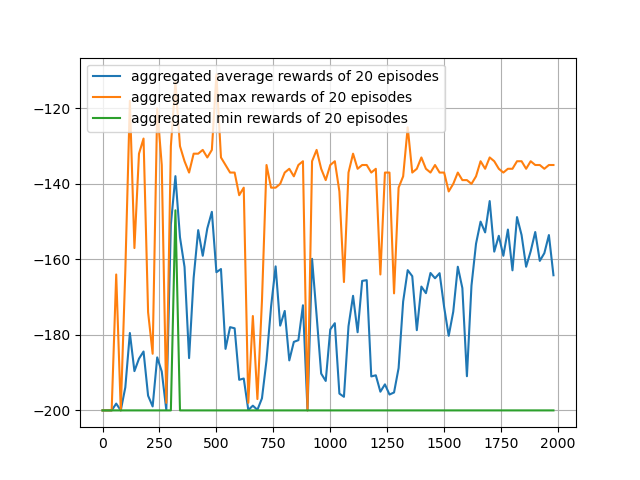
\includegraphics[width=0.7\linewidth]{reward}
	\caption{average rewards}
	\label{fig:reward}
\end{figure}


\subsection*{b)}


\end{document}
